\documentclass[10pt]{report}
\usepackage{polyglossia}
\usepackage{amsmath}
\usepackage{graphicx}
\usepackage{subcaption}
\usepackage{tikz}
\usepackage{circuitikz}
\usepackage{xcolor}
\usepackage{eso-pic,graphicx,transparent}
\usepackage{multicol}
\usepackage{fancyhdr}




\pagestyle{fancy}

\chead{Fibonacci  Numbers}
\lhead{}
\rhead{}
\cfoot{\thepage}
\lfoot{\textbf{\textit{\textcolor{red}{Marian} \textcolor{blue}{College} \textcolor{brown}{Kuttikkanam}} }}
\rfoot{}



\usepackage{fontspec}
 \setdefaultlanguage{malayalam}
\setmainfont[Script=Malayalam, HyphenChar="00AD]{Rachana}

\usepackage{eso-pic}



%
%\setdefaultlanguage{malayalam}
%\setmainfont[Script=Malayalam, HyphenChar="00AD]{Rachana}
\title{\LARGE\textbf{FIBONACCI NUMBERS AND NATURE\\ ഫിബോനാക്കി സംഖ്യകളും പ്രകൃതിയും}}%{LaTex Project} 
\author{Sanjo Varghese \\
 Participant of Scientific Documentation using \LaTeX\ programme \\
 \textbf{ICFOSS}, Government of Kerala
 }
\begin{document}

\maketitle
\pagenumbering{roman}
\tableofcontents
\listoffigures
\listoftables

\chapter{FIBONACCI NUMBERS}
\pagenumbering{arabic}
\section{Leonardo Fibonacci}

	\begin{multicols}{2}
Leonardo Fibonacci, also called Leonardo Pisano or Leonard of Pisa, was the most  outstanding mathematician of the European Middle Ages. Little is known about his life except for the few facts he gives in his mathematical writings. Ironically, none of his contemporaries mention him in any document that survives.

Fibonacci was born around 1170 into the Bonacci family of Pisa, a prosperous mercantile center. ("Fibonacci" is a contraction of "Filius Bonacci," son of Bonacci.) His father Guglielmo (William) was a successful merchant, who wanted his son to follow his trade.

Around 1190, when Guglielmo was appointed collector of customs in the Algerian city of Bugia, he brought Leonardo there to learn the art of computation. In Bougie, Fibonacci received his early education from a Muslim schoolmaster, who introduced him to the Indo-Arabic numeration system and Indo-Arabic computational techniques. He also introduced Fibonacci to a book on algebra, Hisab al-jabr walmuqabalah, written by the Persian mathematician, al-Khowarizmi.  

As an adult, Fibonacci made frequent business trips to Egypt, Syria, Greece, France, and Constantinople, where he studied the various systems of arithmetic then in use, and exchanged views with native scholars. He also lived for a time at the court of the Roman Emperor, Frederick II (1194-1250), and engaged in scientific debates with the Emperor and his philosophers.

Around 1200, at the age of about 30, Fibonacci returned home to Pisa. He was convinced of the elegance and practical superiority of the Indo-Arabic system over the Roman numeration system then in use in Italy. In 1202, Fibonacci published his pioneering work, Liber Abaci The Book of the Abacus.) (The word abaci here does not refer to the hand calculator called an abacus, but to computation in general.) Liber Abaci was devoted to arithmetic and elementary algebra; it introduced the Indo-Arabic numeration system and arithmetic algorithms to Europe. 

\end{multicols}
	
	In fact, Fibonacci demonstrated in this book the power of the Indo-Arabic system more vigorously than in any mathematical work up to that time. Liber Abaci's  explain the
major contributions to algebra by al-Khowarizmi and another Persian mathematician, Abu Kamil . Six years later, Fibonacci revised Liber Abaci and dedicated the second edition to Michael Scott, the most famous philosopher and astrologer at the court of Frederick II.

After Liber Abaci, Fibonacci wrote three other influential books. Practica Geometriae {Practice of Geometry), written in 1220, is divided into eight chapters  and is dedicated to Master Domonique, about whom little is known. This book skillfully presents geometry and trigonometry with Euclidean rigor and some originality. Fibonacci employs algebra to solve geometric problems and geometry to solve algebraic problems, a radical approach for the Europe of his day.

To find a solution of the cubic equation $x^3 + 2x^2 +10x- 20 = 0$  . Fibonacci showed geometrically that it has no solutions of the form $\sqrt{a+\sqrt{b}}$, but gave an approximate solution, 1.3688081075, which is correct to nine decimal places. 




\section{Fibonnacci Numbers}
The numbers in the bottom row are called Fibonacci numbers, and the number sequence $1, 1, 2, 3, 5, 8, \ldots$ is the Fibonacci sequence.  The Fibonacci sequence is one of the most intriguing number sequences, and it
continues to provide ample opportunities for professional and amateur mathematicians to make conjectures and to expand the mathematical horizon.

\subsection{Recursive Definition}
This observation yields the following recursive definition of the $n^{th}$  Fibonacci number, $F_n $ :
 \[F_1=F_2=1\]
 \[
 F_n=F_{n-1}+F_{n-2} \quad n\geq 3
 \]

\chapter{Fibonnacci Numbers in  NAature}
Interestingly enough, the amazing Fibonacci numbers occur in quite unexpected places in nature.

\subsection{Fibonacci and the Earth}

Zerger observed that the equatorial diameter of the earth in miles is approximately the product of two alternate Fibonacci numbers, and that this in kilometers is approximately the product of three consecutive
Fibonacci numbers: 
$$55 \cdot 144 = 7920 \mbox{ miles and }   89 \cdot 144 = 12,816 \mbox{ kilometers} $$

\subsection{Fibonacci and Illinois}
In 1992, Zerger discovered some astonishing occurrences of Fibonacci numbers in relation to the state of Illinois :
\begin{itemize}
 \item Illinois was admitted to the Union on the 3rd of December.
 \item Illinois is the fifth largest state, according to the 1990 census.
 \item Illinois' name consists of 8 letters.
 \item Illinois is the thirteenth state, when the states are arranged alphabetically.
 \item Illinois was the twenty-first state admitted to the Union. The postal abbreviation
IL is formed with the ninth and twelfth letters : $9 + 12 = 21$.
 \item Interstate 55 begins in Chicago and roughly follows the 89th parallel to New Orleans.
\end{itemize}

\subsection{Fibonacci and Flowers}
The number of petals in many flowers is often a Fibonacci number. For instance, count the number of petals in the flowers pictured in Figure \ref{fig-1} Enchanter's nightshade has two petals, iris and trillium three, wild rose five, and delphinium and cosmos eight. Most daisies have 13, 21, or 34 petals; there are even daisies with 55 and 89 petals. Table \ref{tab-1} lists the Fibonacci number of petals in an assortment of flowers. Although some plants, such as buttercup and iris, always display the same number of petals, some do not. For example, delphinium blossoms sometimes have 5 petals and
sometimes 8 petals, and some Michaelmas daisies have 55 petals, while some have 89 petals. The cross section of an apple reveals a pentagonal shape with five pods. The starfish, with five limbs, also exhibits a Fibonacci number

\begin{figure}
\centering
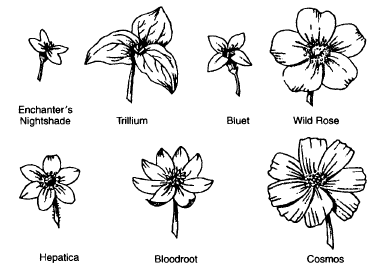
\includegraphics[height=5 cm, width=8cm]{flowers.png}
\caption{Flowers}
\label{fig-1}
\end{figure}

\begin{table}
	\centering
	\begin{tabular}{ | c |  p{7 cm} | c | } 
		\hline
		No. & Plant  &Number of Petals
		 \\ 
		\hline
		1&Enchanter's nightshade &2 \\
		\hline
2&  Iris, lilly & 3 \\
\hline
3 & Buttercup, columbine, delphinium, larkspur, wall lettuce & 5 \\
\hline
4 & Celandine, delphinium, field senecio, squalid senecio & 8 \\
\hline
5 & Chamomile, cineraria, corn marigold, double delphinium, globeflower & 13 \\
\hline
6 & Aster, black-eyed Susan, chicory, doronicum, helenium, hawkbit & 21 \\
\hline
7& Daisy, gailliardia, plantain, pyrethrum, hawkweed & 34 \\		
	\hline
	\end{tabular}
\caption{Flowers with Fibonacci number}
\label{tab-1}
	\end{table}
\subsection{Fibonacci  and Sunflowers}
Mature sunflowers display Fibonacci numbers in a unique and remarkable way. The seeds of the flower are tightly packed in two distinct spirals, emanating from the center of the head to the outer edge figure \ref{fig-2}. One goes clockwise and the other counterclockwise. Studies have shown that although there are exceptions, the number of spirals, by and large, is adjacent Fibonacci numbers; usually, they are 34 and 55. Hoggatt reports a large sunflower with 89 spirals in the clockwise direction and 55
in the opposite direction, and a gigantic flower with 144 spirals clockwise and 89 counterclockwise. It is interesting to note that Br. Alfred Brousseau once gave Hoggatt a sunflower with 123 clockwise spirals and 76 counterclockwise spirals, two adjacent Lucas spirals.

\begin{figure}[h!]
	\centering
	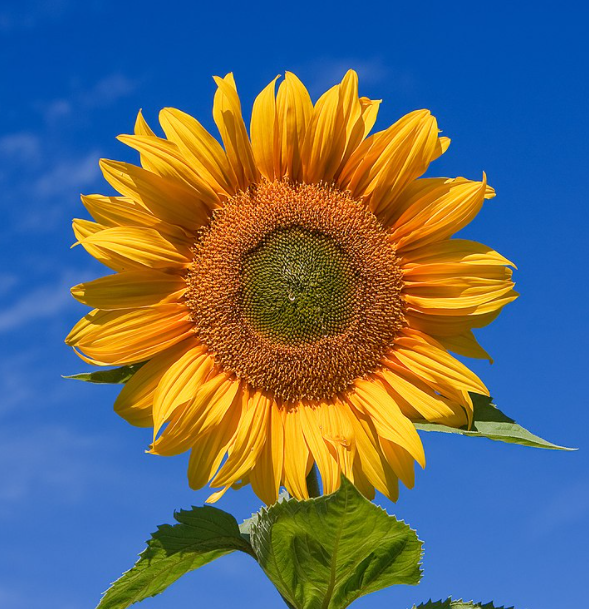
\includegraphics[height=45 mm, width=0.45 \textwidth ]{sunflower.png}
	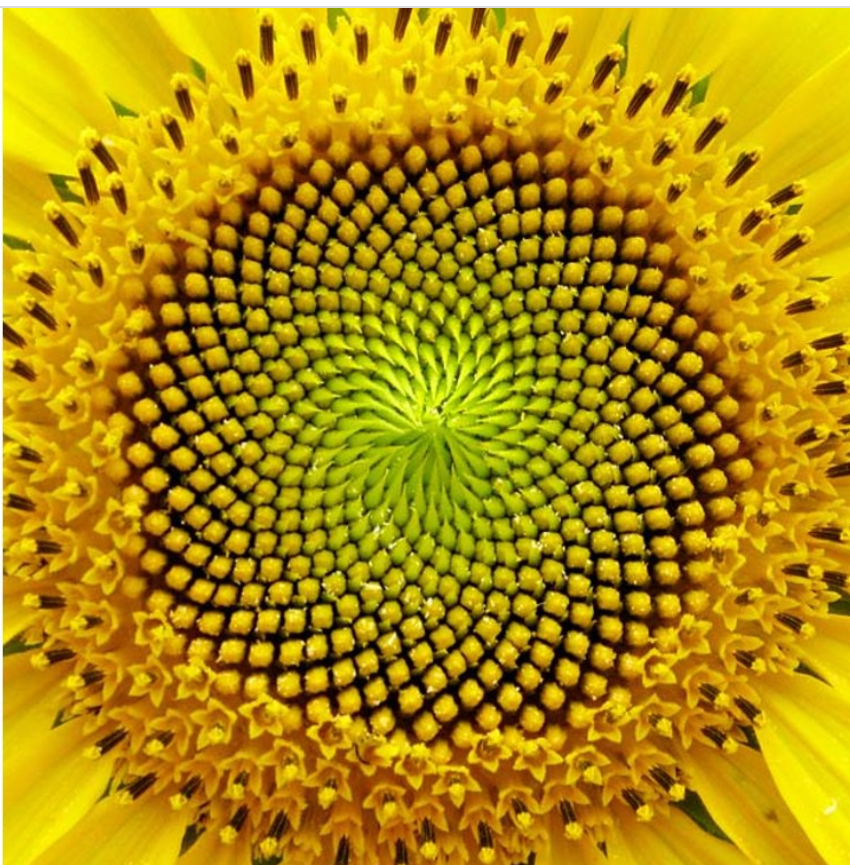
\includegraphics[height=4.5 cm, width=0.45 \textwidth ]{sunflower1.png}
	\caption{Sunflower and its spiral patern}
	\label{fig-2}
\end{figure}
In 1951, John C. Pierce of Goddard College in Massachusetts reported in The
Scientific Monthly that the Russians had grown a sunflower head with 89 and 144 spirals. After reading his article on Fibonacci numbers, Margaret K. O'Connell and Daniel T. O'Connell of South Londonderry, Vermont, examined their sunflowers, raised from seeds from Burpee's. They found heads with 55 and 89 spirals, some with 89 and 144 spirals, and one giant head with 144 and 233 spirals. The latter seems to be a world record.

 

\section{Fibonacci  and Beehive}
Consider two adjacent rows of cells in an infinite beehive, as pictured in Figure \ref{fig-3}. We would like to find the number of paths the bee can take to crawl from one cell to  an adjacent one. It can move in only one general direction, namely, to the right.

Let $b_n$ denote the number of different paths to the $n^{th}$ cell. Since there is exactly one path to cell A (see Fig. \ref{fig-4} ), $b_1 =1$. There are two distinct paths to cell B, as Figure 3.14 shows. So $b_2= 2$. There are three different paths the bee can take to cell  C, so $b_3  = 3$. There are five distinct paths the bee can take to cell D,  as Figure \ref{fig-5} shows. Consequently, $b_4 = 5$, likewise,  $b_5= 8$.

\pagecolor{yellow!40}
\begin{figure}[!ht]
	\centering
	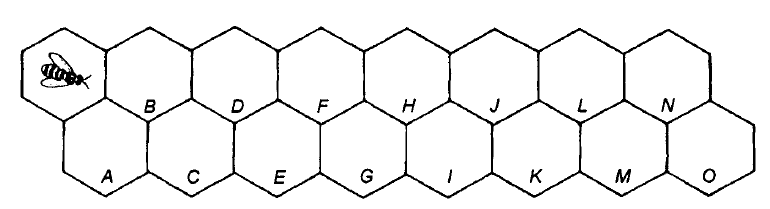
\includegraphics[height=3cm, width=10cm ]{bee.png}
	\caption{Beehive}
	\label{fig-3}
\end{figure}
\begin{figure}[!ht]
	\centering
	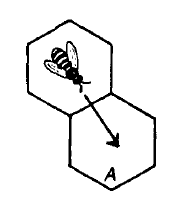
\includegraphics[height=3cm, width= 3cm ]{bee1.png}
	\caption{Beehive cell 1}
	\label{fig-4}
\end{figure}
\begin{figure}[h!]
	\centering
	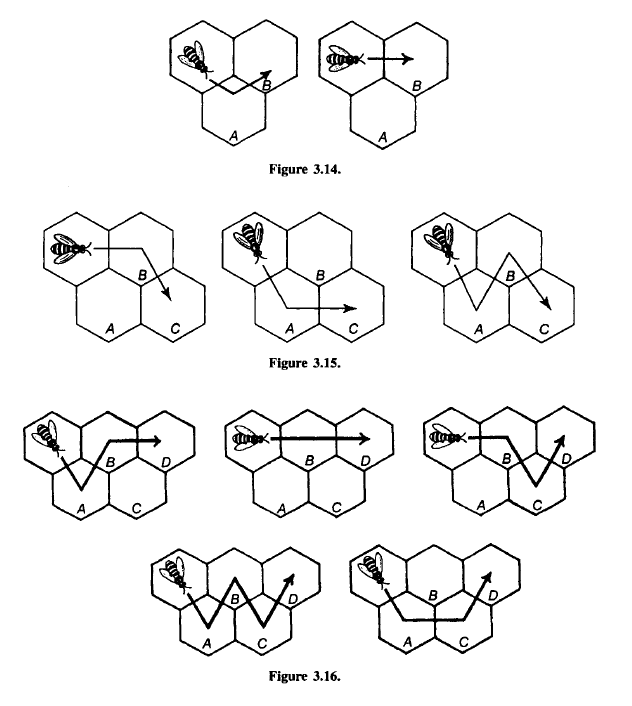
\includegraphics[height=8cm, width= 9cm ]{bee2.png}
	\caption{Beehive cells}
	\label{fig-5}
\end{figure}

\chapter{Usage of \LaTeX\ in Mathematics, creating images  and Circuits}
\section{Equations}
\begin{itemize}
		\item Differential equation : 
		$\displaystyle\frac{d^2y}{dx^2} + \frac{dy}{dx} - 6y = 0 $
	\item Integration :  
	\begin{enumerate}
		\item $\int  \cos x \ dx = \sin x + c $
		\item $\int_{0}^{\frac{\pi}{2}} \cos x \ dx = 1 $
	\end{enumerate}
	\item Matrix
	\begin{center}
		$\begin{bmatrix}
			4 & 2 & 7\\
			5 & 3 & 1
		\end{bmatrix}$
	\end{center}
\end{itemize}


\section{Multi figures}
\subsection{Sample electric Circuit}
\begin{circuitikz}
	\draw (0,0)
	to[V,v=$U_q$] (0,2) % The voltage source
	to[short] (2,2)
	to[R=$R_1$] (2,0) % The resistor
	to[short] (0,0);
	\draw (2,2)
	to[short] (4,2)
	to[L=$L_1$] (4,0)
	to[short] (2,0);
\end{circuitikz}
\newpage
\subsection{Multiple Figures using subfigure}

{\centering
	\begin{figure}[h!]
		\centering
		\begin{subfigure}[b]{0.45\textwidth}
			\centering
			{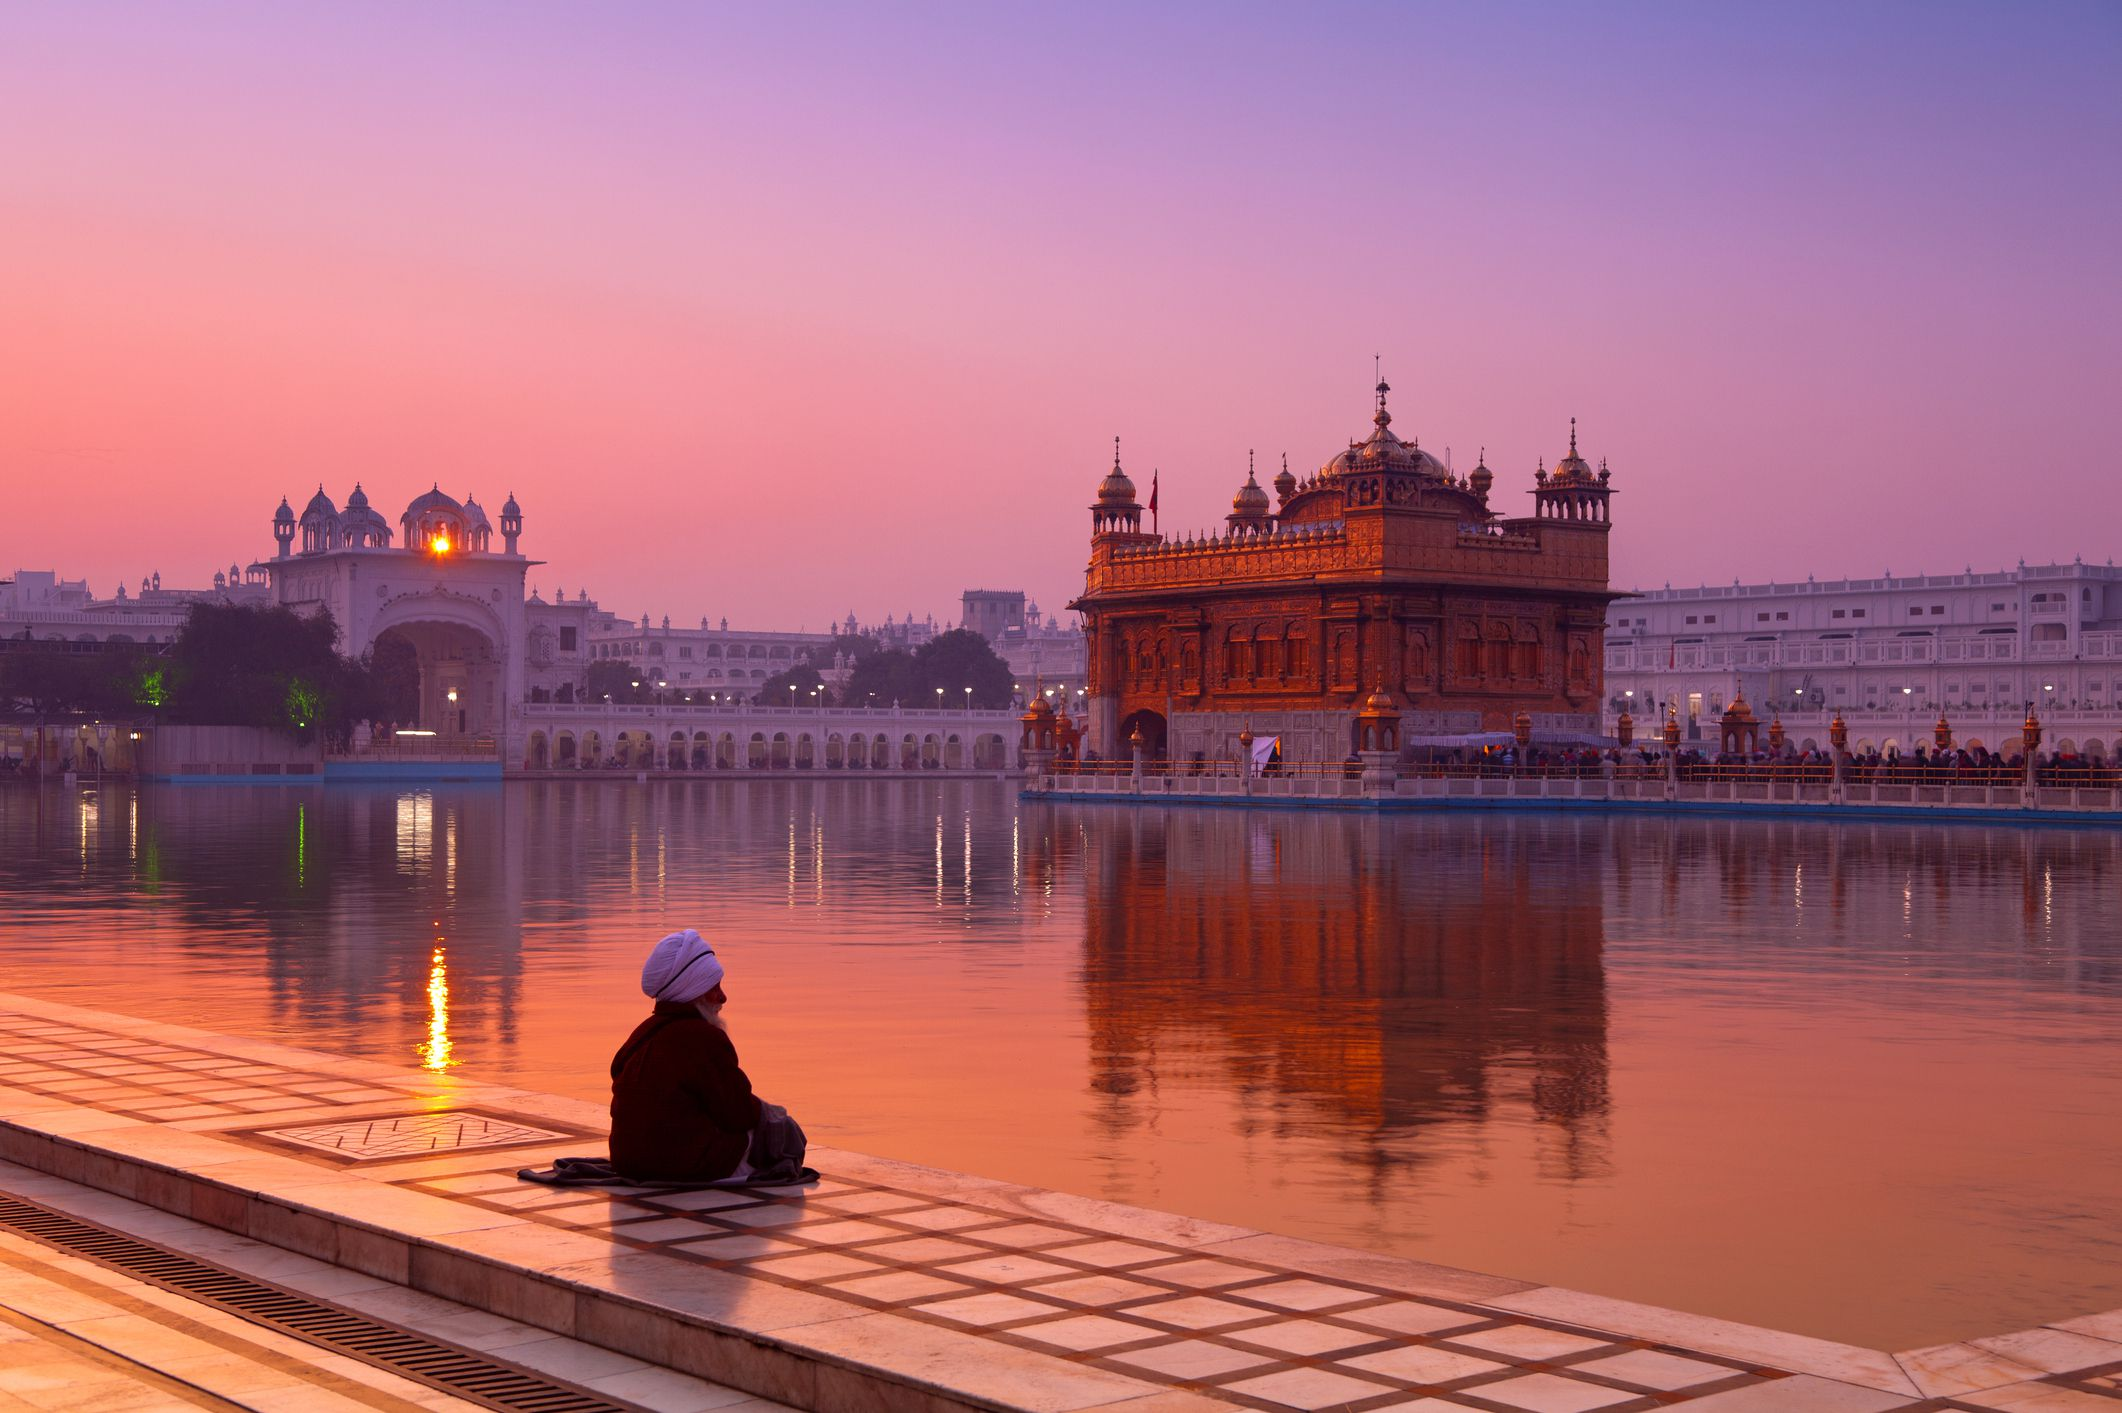
\includegraphics[height=4  cm,width=5.5 cm]{pic1.jpg}}
			\caption{Image-1}
			\label{aa}
		\end{subfigure}
		\begin{subfigure}[b]{0.45\textwidth}
			\centering
			{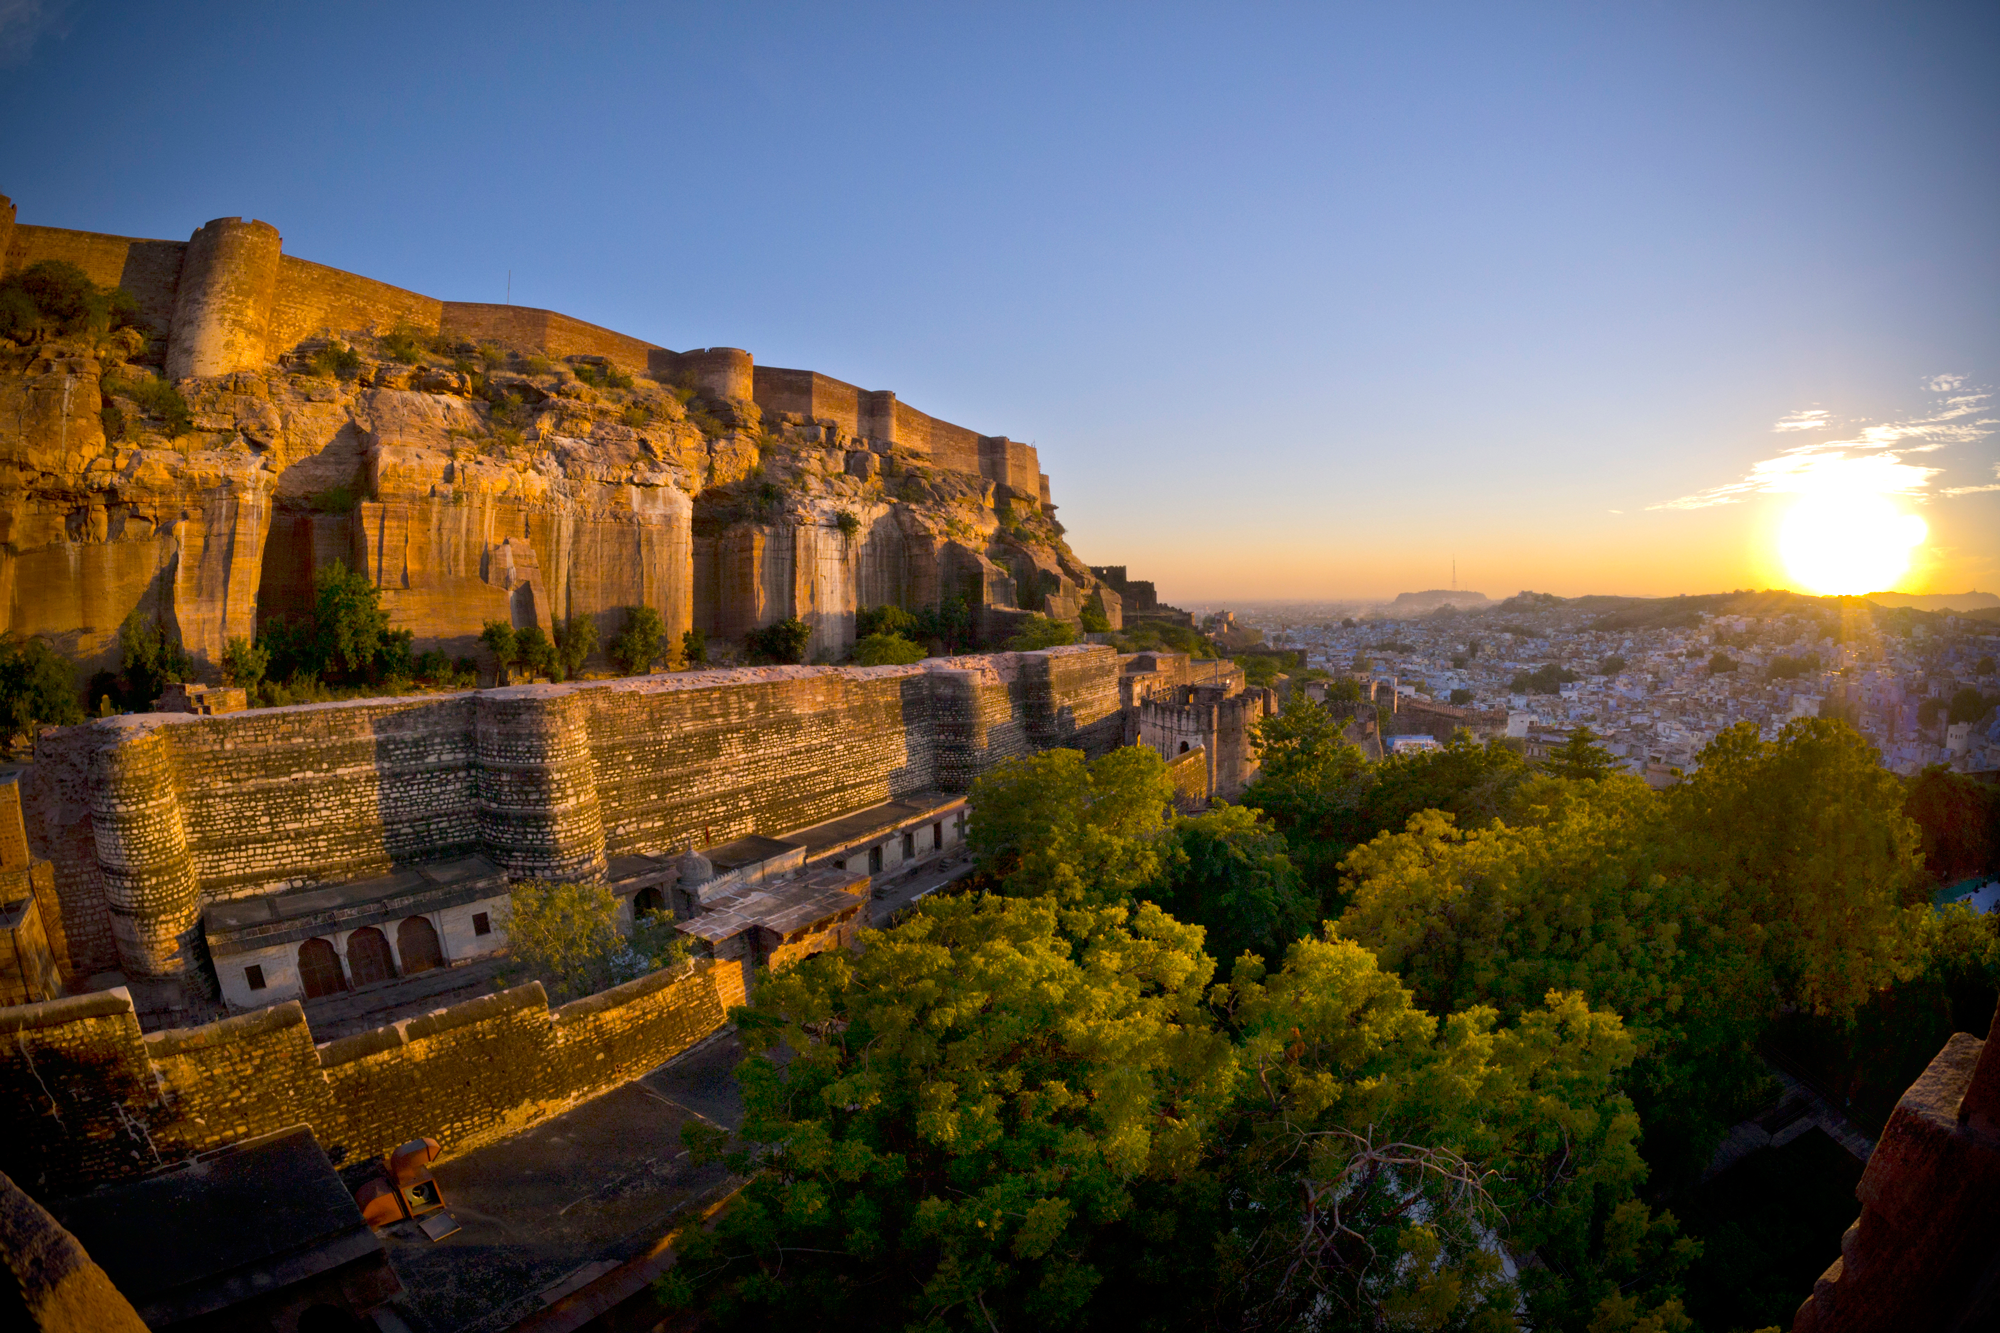
\includegraphics[height=4 cm,width=5.5 cm]{pic3.png}}
			\caption{Image-2}
			\label{aa-B}
		\end{subfigure}
		\begin{subfigure}[b]{0.45\textwidth}
		\centering
		{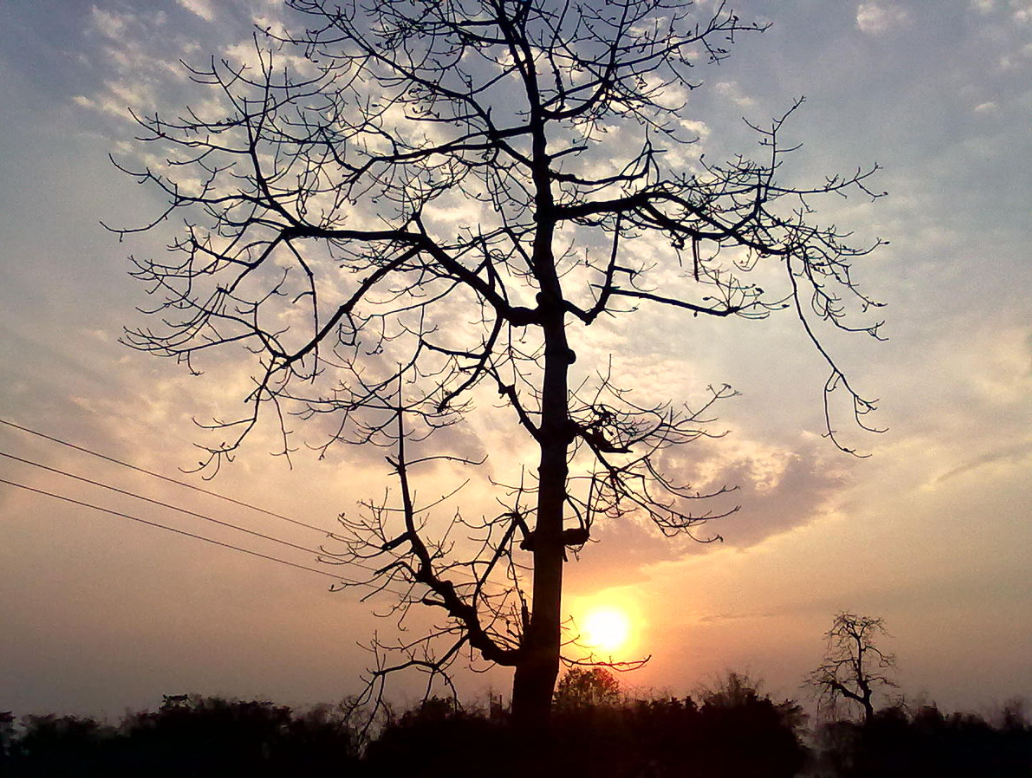
\includegraphics[height=4  cm,width=5.5 cm]{nature.png}}
		\caption{Image-3}
		\label{aa}
	\end{subfigure}
	\begin{subfigure}[b]{0.45\textwidth}
		\centering
		{\includegraphics[height=4 cm,width=5.5 cm]{aa.jpg}}
		\caption{Image-4}
		\label{aa-B}
	\end{subfigure}
		\caption{Multiple images using subfig  enviornment}
		\label{aa}
	\end{figure}
}


\end{document}